\section{Introduction}
\label{sec:introduction}

An increasing number of swarm applications rely on heavy computation tasks,
notably machine learning (ML) applications. For example, Microsoft
SeeingAI~\cite{seeingai} is a talking camera for the blind and low vision
community that describes nearby people, text, objects, etc. Wearable cognitive
assistant~\cite{ha2014towards} uses wearable devices, such as Google Glass, for
deep cognitive assistance, e.g., offering hints for social interaction via
real-time scene analysis.

While there is a staggering collection of research focusing on model
\textit{training} for these tasks, for swarm applications, they perform the
\textit{inference} step of machine learning: it uses a trained model to make a
prediction given an input, such as visual~\cite{googlelens, ha2014towards,
  seeingai}, audio~\cite{alexa, applesiri, cortana}, and sensory
information~\cite{laput2017synthetic, lu2010jigsaw}. Inference has received
relatively little attention, especially on edge and end devices.

One important challenge in swarm applications is to bound the response time,
which affects user experience significantly in these human-in-the-loop
systems. Previous usability studies~\cite{nielsen1994usability,
  schneiderman1998designing} have measured the effect of different end-to-end
response times:

\begin{itemize}[noitemsep, topsep=0pt]
\item 100 ms gives the feeling of instantaneous response.
\item 1 second keeps the user's flow of thought but users can sense the delay.
\item A few seconds' delay creates an unpleasant user experience.
\end{itemize}

Achieving bounded response times (BRT) on swarm devices has remained
challenging. Swarm devices are extremely heterogeneous and many are resource
constrained (see \autoref{tab:embedded}). Heavy computations are often beyond
the capabilities of cheap end devices. For example, state-of-the-art object
detection algorithm easily takes several seconds on modern
smartphones~\cite{chen2015glimpse}.

To compensate resource-constrained devices, prior work explores
offloading~\cite{chun2011clonecloud,cuervo2010maui} to the cloud or the edge
that hosts machine learning models and performs heavy computation. Despite their
powerful computing capability and more available resources, e.g., special
hardware like GPU and TPU~\cite{jouppi2017datacenter}, these machines suffer
from increased network latency and service overload (\autoref{fig:edge}). As a
result, they are often unable to meet response time goals consistently.

Another technique for low latency is to use redundant requests. By initiating
multiple requests across a diverse set of resources and using the first result
that completes, redundancy is effective to address the variability in network
delays~\cite{gordon2015accelerating, vulimiri2013low} and slow servers (known as
straggler mitigation in the cloud~\cite{dean2013tail,
  ananthanarayanan2013effective}). However, existing works treat these resources
equally and execute the same task on each platform, a poor match for the
heterogeneous swarm space.

We make the observation that for a particular task, there are many options:
different algorithms or tunable parameters for the same algorithm. These options
result in different processing times and application accuracy. If we can adapt
the computation by choosing an option that matches the capability of the device
or satisfy the deadline requirement, we can achieve bounded response times.

The idea of adapting to machines is illustrated in \autoref{fig:dr}. It builds
on top of redundancy but addresses, or rather leverages, the heterogeneity of
swarm devices.  On-device processing can use a simple algorithm if the device is
resource constrained. The device also sends redundant requests to other servers,
e.g., the edge and/or the cloud. Each request contains a service-level objective
(SLO) that describes the deadline and accuracy demand. Upon receiving the
request, the server would admit or reject the request based on the network
delays and its workload. Because of the redundancy, rejection is fine. This is
different from traditional web serving where the server is the single point of
source. At last, the device would use the first response that completes.

\begin{figure}
  \centering
  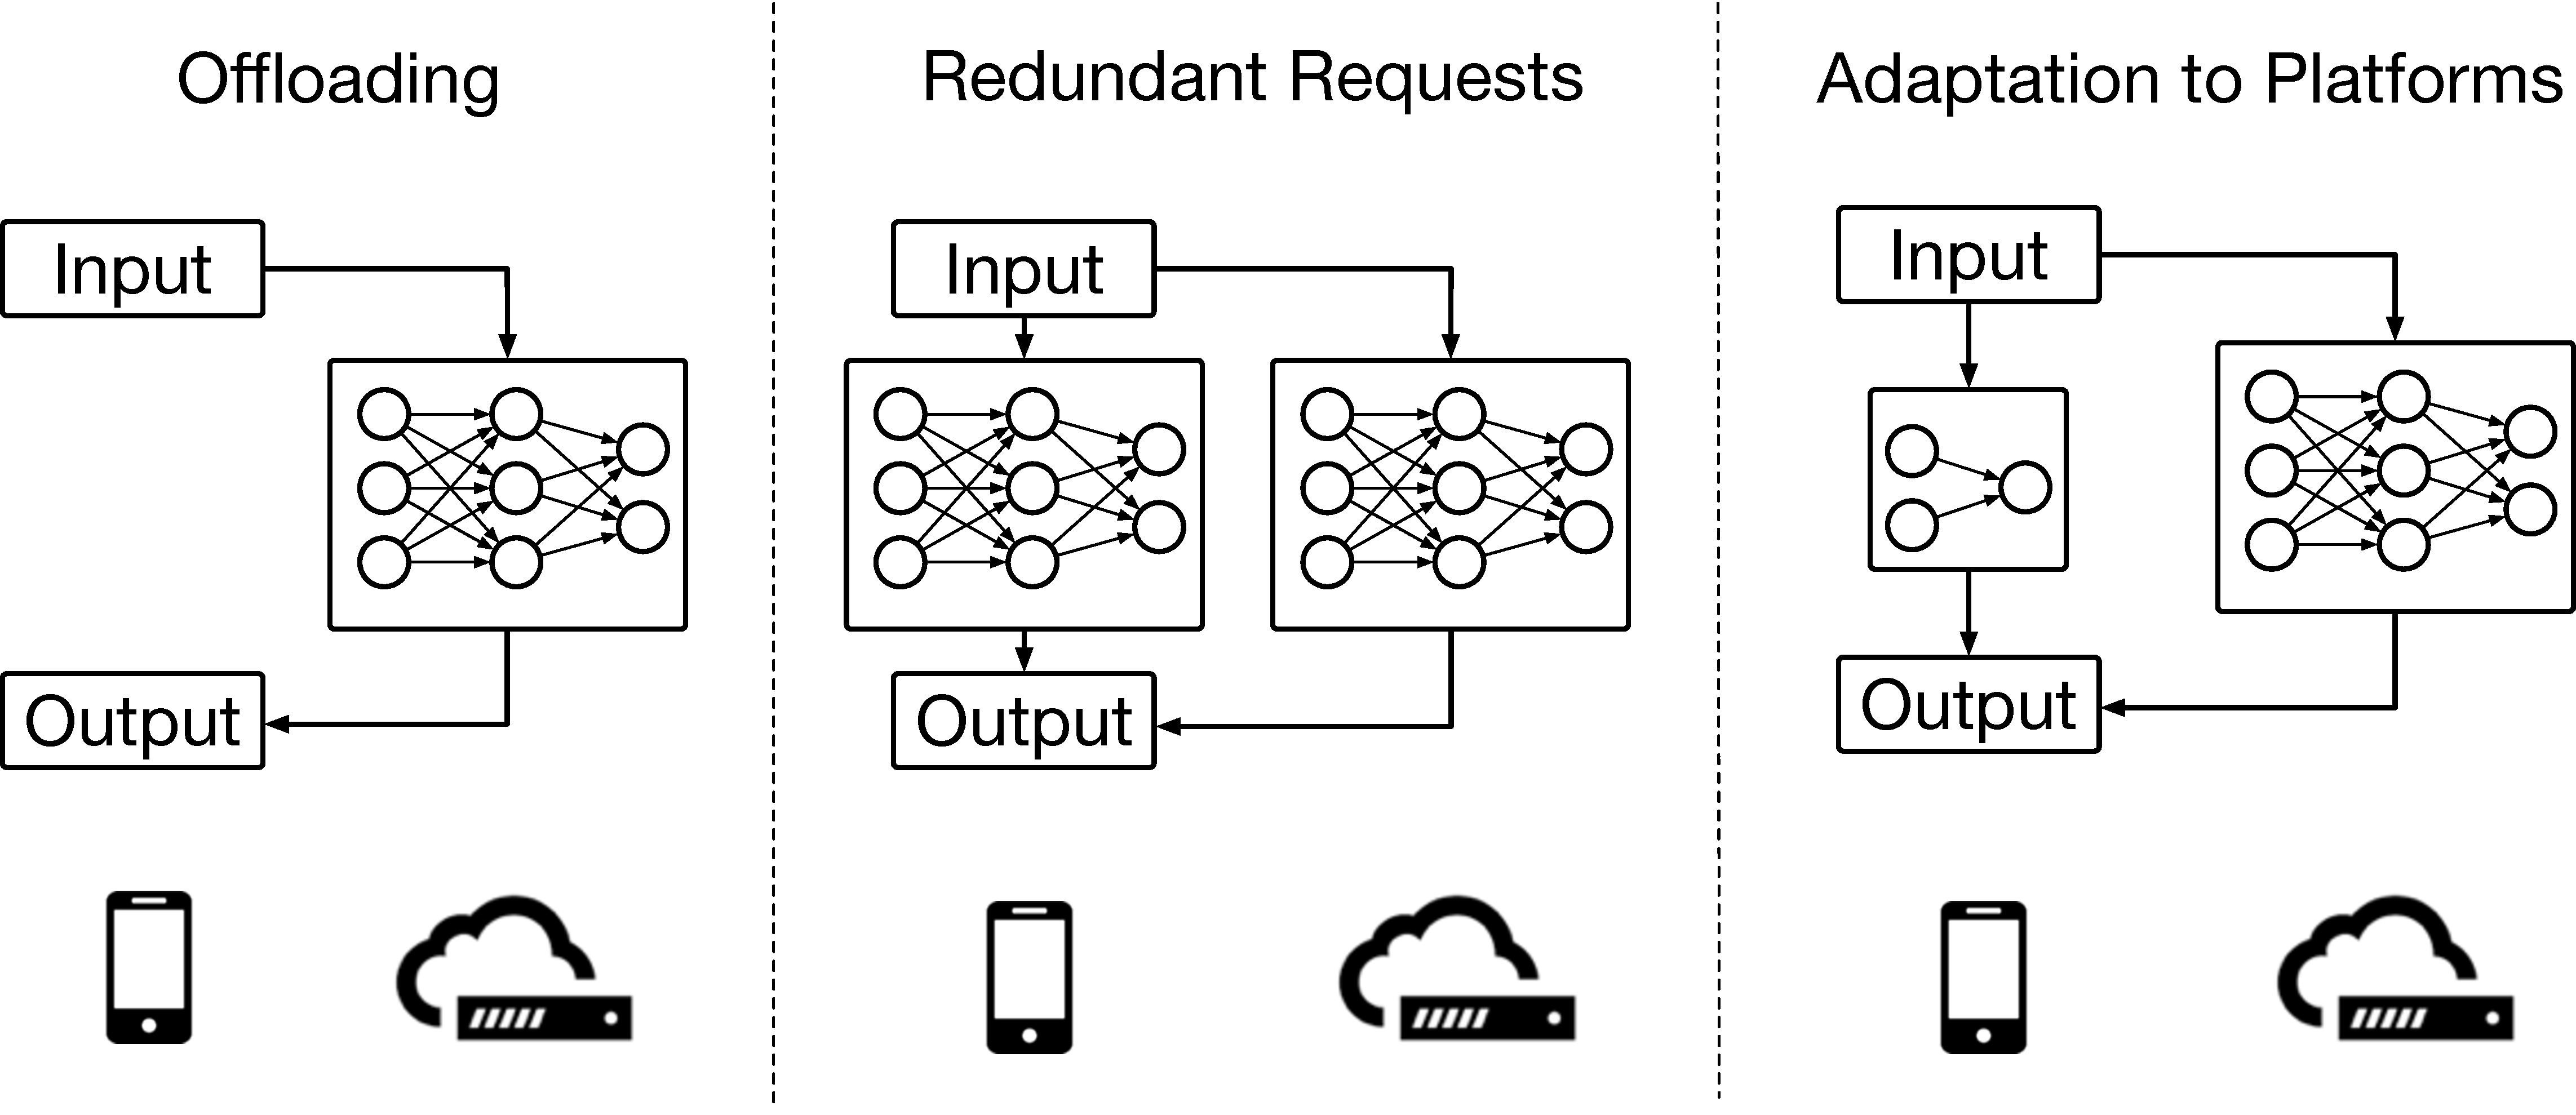
\includegraphics[width=0.8\columnwidth]{figures/dr.pdf}
  \caption{Illustration of offloading, redundant requests and compute
    adaptation.}
  \label{fig:dr}
\end{figure}

The key to enable adaptation lies in building an accurate performance model that
characterized the processing times and accuracy trade-off for a particular
task. We take a data-driven approach by measuring processing times and accuracy
for a given set of training data. We call this process \emph{profiling} and the
resulting performance model is \emph{the profile}.

Efficient profiling is challenging given the large space formed by the
combination of algorithms, parameters, and machines. We need to profile each
algorithms individually. For a single algorithm, it may have a huge parameter
space. For example, cascading classifiers in computer vision tasks have
configurable convolution window size, scale factor, and minimum neighbor for non
maximum suppression. Exhaustive profiling in this space is prohibitively
expensive (see \autoref{fig:vj-tradeoff}). Because processing times depend on
the devices, the profile is different across devices. It is infeasible to
profile all hardware platforms because of the staggering number of devices and
their availability, or rather lack of, at development time.

In this chapter, we first describe our programming abstraction based on macro
annotations. Developers only need small modifications to their existing code to
express adaptation options for different algorithms and parameters. We then
discuss techniques to build the performance model efficiently. Our profiling
makes the following contribution,

\begin{enumerate}[noitemsep, topsep=0pt]
\item To address the large parameter space, we use Bayesian Optimization (BO)
  for profiling. For Viola-Jones face detector, an exhaustive approach requires
  more than 4000 samples while BO learns the profile with around 80
  samples---more than 50$\times$ fewer samples.
\item We make the observation that only processing times vary across devices. As
  a result, it is sufficient to only measure the processing times for
  configurations from the Pareto-optimal set. The profile transfer eliminates
  the need to get all training data, evaluate the algorithm for all data, and
  run BO engine.
\end{enumerate}

%%% Local Variables:
%%% mode: latex
%%% TeX-master: "../compute"
%%% End:
